% ----------------------------------------------------------------- %
%             The Speech Signal Processing Toolkit (SPTK)           %
%             developed by SPTK Working Group                       %
%             http://sp-tk.sourceforge.net/                         %
% ----------------------------------------------------------------- %
%                                                                   %
%  Copyright (c) 1984-2007  Tokyo Institute of Technology           %
%                           Interdisciplinary Graduate School of    %
%                           Science and Engineering                 %
%                                                                   %
%                1996-2017  Nagoya Institute of Technology          %
%                           Department of Computer Science          %
%                                                                   %
% All rights reserved.                                              %
%                                                                   %
% Redistribution and use in source and binary forms, with or        %
% without modification, are permitted provided that the following   %
% conditions are met:                                               %
%                                                                   %
% - Redistributions of source code must retain the above copyright  %
%   notice, this list of conditions and the following disclaimer.   %
% - Redistributions in binary form must reproduce the above         %
%   copyright notice, this list of conditions and the following     %
%   disclaimer in the documentation and/or other materials provided %
%   with the distribution.                                          %
% - Neither the name of the SPTK working group nor the names of its %
%   contributors may be used to endorse or promote products derived %
%   from this software without specific prior written permission.   %
%                                                                   %
% THIS SOFTWARE IS PROVIDED BY THE COPYRIGHT HOLDERS AND            %
% CONTRIBUTORS "AS IS" AND ANY EXPRESS OR IMPLIED WARRANTIES,       %
% INCLUDING, BUT NOT LIMITED TO, THE IMPLIED WARRANTIES OF          %
% MERCHANTABILITY AND FITNESS FOR A PARTICULAR PURPOSE ARE          %
% DISCLAIMED. IN NO EVENT SHALL THE COPYRIGHT OWNER OR CONTRIBUTORS %
% BE LIABLE FOR ANY DIRECT, INDIRECT, INCIDENTAL, SPECIAL,          %
% EXEMPLARY, OR CONSEQUENTIAL DAMAGES (INCLUDING, BUT NOT LIMITED   %
% TO, PROCUREMENT OF SUBSTITUTE GOODS OR SERVICES; LOSS OF USE,     %
% DATA, OR PROFITS; OR BUSINESS INTERRUPTION) HOWEVER CAUSED AND ON %
% ANY THEORY OF LIABILITY, WHETHER IN CONTRACT, STRICT LIABILITY,   %
% OR TORT (INCLUDING NEGLIGENCE OR OTHERWISE) ARISING IN ANY WAY    %
% OUT OF THE USE OF THIS SOFTWARE, EVEN IF ADVISED OF THE           %
% POSSIBILITY OF SUCH DAMAGE.                                       %
% ----------------------------------------------------------------- %
\hypertarget{fftr}{}
\name{fftr}{FFT for real sequence}{signal processing}

\begin{synopsis}
 \item[fftr] [ --l $L$ ] [ --m $M$] [ --\{ A $|$ R $|$ I $|$ P \} ] [ --H ]
             [ {\em infile} ] 
\end{synopsis}

\begin{qsection}{DESCRIPTION}
{\em fftr} uses the Fast Fourier Transform (FFT) algorithm 
to calculate the Discrete Fourier Transform (DFT) 
of real-valued input data in {\em infile} (or standard input), 
and sends the result to standard output. 
To specify the FFT size, --l option can be used.
Also, --m option can be used to pad the input data with zeros.
When $M + 1 \leq L$,  the input data is padded
with $L - M - 1$ zeros. When $M + 1 > L$, {\em fftr} terminates
with error messages.
The input and output data is in float format, 
arranged as below.
\begin{displaymath}
\begin{array}{lll}
\mbox{Input sequence} & 
\overbrace{\framebox[4.5cm]{$x_0, x_1, \ldots, x_{M}, 0,
                                        \ldots,0$}}^{L}  & \\
                & \makebox[4.5cm]{0\hfill $L-1$} &
\end{array}
\end{displaymath}
\begin{displaymath}
\begin{array}{lll}
\mbox{Output sequence} & \overbrace{\framebox[4.5cm]{real part}}^{L} &
           \overbrace{\framebox[4.5cm]{imaginary part}}^{L} \\
                & \makebox[4.5cm]{0\hfill $L-1$} &
                \makebox[4.5cm]{0\hfill $L-1$}
\end{array}
\end{displaymath}
\end{qsection}

\begin{options}
        \argm{l}{L}{FFT size power of 2}{256}
        \argm{m}{M}{order of sequence}{L-1}
        \argm{A}{}{output magnitude}{FALSE}
        \argm{R}{}{output only real part}{FALSE}
        \argm{I}{}{output only imaginary part}{FALSE}
        \argm{P}{}{output power spectrum}{FALSE}
        \argm{H}{}{output half size}{FALSE}
\end{options}

\begin{qsection}{EXAMPLE}
In the example below, a sine wave is passed through a Blackman window,
its DFT is evaluated and the magnitude is plotted:
\begin{quote}
  \verb!sin -p 30 | window | fftr -A | fdrw | xgr!
\end{quote}
\begin{center}
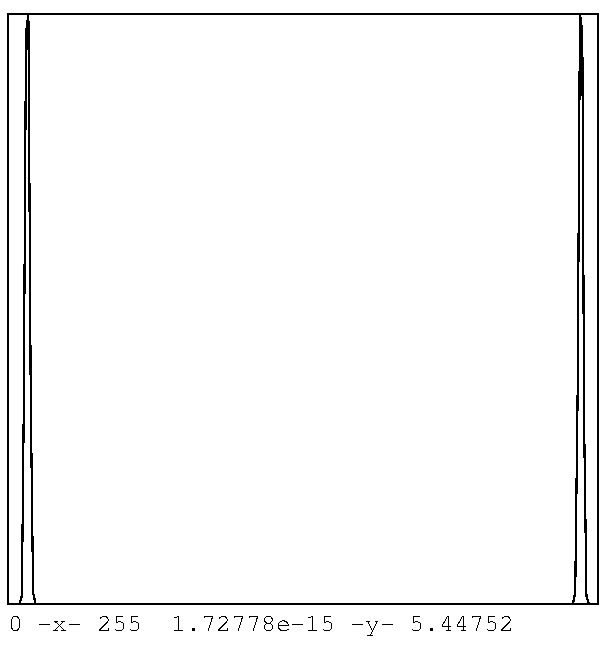
\includegraphics[width=6cm]{fig/fftr.pdf}
\end{center}

\end{qsection}

\begin{qsection}{SEE ALSO}
\hyperlink{fft}{fft},
\hyperlink{fft2}{fft2},
\hyperlink{fftr2}{fftr2},
\hyperlink{ifft}{ifft}
\hyperlink{ifftr}{ifftr}
\hyperlink{ifft2}{ifft2}
\hyperlink{spec}{spec},
\hyperlink{phase}{phase}
\end{qsection}
